% describe the modification of the Impact algorithm for heaps

% describe the standard Impact algorithm
% \section{Heap Impact Algorithm}
\label{ch:heap-impact-algorithm}
%

Building on top of the framework defined in \autoref{ch:background}, \autoref{ch:impact-algorithm}, and \autoref{ch:heap-patterns}, we can define \verifier, by modifying the \impact algorithm to work for heap-manipulating programs. In this section, we first define the three steps of \impact, that is \expand, \cover, and \refine. Then we describe an invariant-learning procedure that retrieves patterns from an Oracle, thereby completing the description of the algorithm.

\begin{algorithm}[ht]
  % Declare functions
  \SetKwFunction{procexpand}{EXPAND}

  % Declare sub-program markers.
  \SetKwProg{myproc}{Procedure}{}{}

  % expand
  \myproc{\procexpand{$v \in V$}:}{
    %
    \If{$v$ is an uncovered leaf}{
        \ForEach{action $(M_v(v),T,m) \in \Delta$}{
        add a new vertex $w$ to $V$ and a new edge $(v,w)$ to $E$; \\
        set $M_v(w) \leftarrow m$ and $\psi(w) \leftarrow 1_D$; \\
        set $M_e(v,w) \leftarrow T$;
      }
    }
  }
  \caption{$\expand$: takes as input a vertex $v \in V$ and expands the control flow graph based on all actions available at that vertex.}
  \label{alg:heap-expand}
\end{algorithm}

\begin{algorithm}[ht]
  % Declare functions
  \SetKwFunction{procrefine}{REFINE}

  % Declare sub-program markers.
  \SetKwProg{myproc}{Procedure}{}{}

  % expand
  \myproc{\procrefine{$v \in V$}:}{
    %
    \If{$M_v(v) = l_f$ and $\psi(v) \not\equiv (\false, 0_D)$}{
      let $\pi = (v_0, T_0, v_1) \cdots (v_{n-1}, T_{n-1}, v_n)$ be the unique path from $\epsilon$ to $v$ \\
      let $\hat{A_0},\cdots,\hat{A_n}$ = \seplearner($\mathcal{U}(\pi)$) \\
      \eIf{$\hat{A_0},\cdots,\hat{A_n}$ is a valid interpolant}{
          \For{$i = 0 \cdots n$}{
          let $\phi = \hat{A}_i^{\langle -i \rangle}$ \\
          \If{$\psi(v_i) \nvDash \phi$}{
            remove all pairs $(\cdot, v_i)$ from $\rhd$; \\
            set $\psi(v_i) \leftarrow \psi(v_i) \land \phi$;
          }
        }
      }
      {
        abort (program is unsafe)
      }
    }
  }
  \caption{$\refine$: takes as input a vertex $v \in V$ at an error location and tags the path from root to $v$ with invariants.}
  \label{alg:heap-refine}
\end{algorithm}

\begin{algorithm}[ht]
  % Declare functions
  \SetKwFunction{proccover}{COVER}

  % Declare sub-program markers.
  \SetKwProg{myproc}{Procedure}{}{}

  % expand
  \myproc{\proccover{$v, w \in V$}:}{
    %
    \If{$v$ is uncovered and $M_v(v) = M_v(w)$ and $v \nvDash w$}{
      \If{$\psi(v) \vDash \psi(w)$}{
        add $(v,w)$ to $\rhd$; \\
        delete all $(x,y) \in \rhd$, s.t. $v \sqsubseteq y$;
      }
    }
  }
  \caption{$\cover$: takes as input vertices $v, w \in V$ and attempts to cover $v$ with $w$.}
  \label{alg:heap-cover}
\end{algorithm}

\section{Postcondition Transforms for Heap Operations}
We first define the operator $\post$, which will be used for generating examples to interact with the Oracle.

% define labeled program unwinding
\begin{defn}
  \label{defn:heap-post-transforms}
  The operator $\post$, which computes the strongest postcondition for a given heap pattern, and action. That is $\post : \heappats \times \mathcal{T} \to \heappats$, where $\mathcal{T}$ is the set of all actions.

  The $\post{*}$ operator can be defined as a repeated application of $\post$ along a given path. More formally, it is $\post{*} : \heappats \times \mathcal{P} \to \heappats$, where $\mathcal{P}$ is a path in the unwinding.
\end{defn}

We also note that the $\post$ operator can be overloaded to work with individual heaps instead of patterns, since single heaps can also be represented using a pattern.

The formal rules for computing $\post$ for each individual action are presented here. We define them for major heap operations that are part of \lang. The formal requirement is that for a heap $h$, pattern $P$, and transition $T$, such that $h \matchedby P$, we must have $\post(h, T) \matchedby \post(P, T)$. Assume that the original pattern is represented by $P = (\nodesnm, \varlblnm, \predlblnm, \edgesnm, \sigma)$, and the pattern after transformation by $\post$ is represented by $P' = (\nodesnm', \varlblnm', \predlblnm', \edgesnm', \sigma')$. We define $P'$ using the definition of $P$, for each possible value of $T$ below. New variables are presented as updates to the values of old variables.

\begin{itemize}
  \item \textbf{ALLOC} ($v := alloc()$): \\
    - $\nodesnm' = \nodesnm \cup \{n\}$ where $n \not \in \nodesnm$ \\
    - $\varlblnm'$ updates $\varlblnm$ such that $\varlblnm'(n, v) = \true$ and $\forall m \neq n, \varlblnm'(m, v) = \false$ \\
    - $\predlblnm'$ updates $\predlblnm$ such that $\forall p, \predlblnm'(n, p) = \maybe$ \\
    - $\edgesnm$ updates $\edgesnm'$ such that $\edgesnm'(n,f,m) = \false$, and $\edgesnm'(m,f,n) = \false$ for all fields $f$ and nodes $m \neq n$ \\
    - $\sigma'$ updates $\sigma$ such that $\sigma'(n) = \true$
  \item \textbf{COPY} ($v1 := v2$): \\
    - $\nodesnm' = \nodesnm$ \\
    - $\varlblnm'$ updates $\varlblnm$ such that $\forall n \in \nodesnm, \varlblnm'(v1, n) = \varlblnm(v2, n)$ \\
    - $\predlblnm' = \predlblnm$ \\
    - $\edgesnm = \edgesnm'$ \\
    - $\sigma' = \sigma$
  \item \textbf{LOAD} ($v1 := v2 \select f$): \\
    - $\nodesnm' = \nodesnm$ \\
    - $\varlblnm'$ updates $\varlblnm$ as follows: \\
      \hspace*{1em} Let $S = \{n \in \nodesnm : \varlblnm(n, v2) = \true \vee \varlblnm(n, v2) = \maybe\}$ \\
      \hspace*{1em} Let $T = \{n \in \nodesnm : \exists s \in S \cdot \edgesnm(s, f, n) = \true \vee \edgesnm(s, f, n) = \maybe\}$ \\
      \hspace*{1em} if $T = \{t\}$ (singleton), then $\varlblnm'(t, v1) = \true$, otherwise $\forall t \in T, \varlblnm'(t, v1) = \maybe$ \\
    - $\predlblnm' = \predlblnm$ \\
    - $\edgesnm = \edgesnm'$ \\
    - $\sigma' = \sigma$
  \item \textbf{STORE} ($v1 \select f := v2$): \\
    - $\nodesnm' = \nodesnm$ \\
    - $\varlblnm' = \varlblnm$ \\
    - $\predlblnm' = \predlblnm$ \\
    - $\edgesnm$ updates $\edgesnm'$ as follows: \\
      \hspace*{1em} Let $S = \{n \in \nodesnm : \varlblnm(n, v1) = \true \vee \varlblnm(n, v1) = \maybe\}$ \\
      \hspace*{1em} Let $T = \{n \in \nodesnm : \varlblnm(n, v2) = \true \vee \varlblnm(n, v2) = \maybe\}$ \\
      \hspace*{1em} $\forall s \in S, t \in T, \edgesnm'(s,f,t) = \maybe$ (and $\true$ if both $S$ and $T$ are singletons) \\
    - $\sigma' = \sigma$
  \item \textbf{PREDICATE} ($\predinstr$): \\
    - $\nodesnm' = \nodesnm$ \\
    - $\varlblnm' = \varlblnm$ \\
    - $\forall n \in \nodesnm, p \in \predvars, \predlblnm'(n,p) = post(p, \predlblnm(n,p), \predinstr)$, where $post$ is a postcondition operator for three-valued predicates \\
    - $\edgesnm = \edgesnm'$ \\
    - $\sigma' = \sigma$
\end{itemize}

\section{Learning Invariants from Positive and Negative Examples}

We note in \autoref{alg:heap-refine} the procedure \seplearner is used, which is the core component of making \impact work for heap-manipulating programs. In this section, we describe this algorithm.

We defined the notion of interpolants in \autoref{sec:interpolants-from-proofs}, and the same applies to \seplearner, which is described in \autoref{alg:invlearner}.

\begin{algorithm}[ht]
  % Declare functions
  \SetKwFunction{procinvlearner}{INVLEARNER}

  % Declare sub-program markers.
  \SetKwProg{myproc}{Procedure}{}{}

  % expand
  \myproc{\procinvlearner{$\mathcal{U}(\pi)$}:}{
    %
    Let $\pi = (l_0, T_0, l_1)(l_1, T_1, l_2) \cdots (l_{n-1}, T_{n-1}, l_n)$ \\
    Set $\hat{A_i} = 1_D, 0 \leq i < n, \hat{A_n} = 0_D$ \\
    Set $H_i^{+} = \{\}, 0 \leq i \leq n$ \\
    Set $H_i^{-} = \{\}, 0 \leq i \leq n$ \\

    \While{$\neg$\isinterpolant($\hat{A},\mathcal{U}(\pi)$)}{
      pick $i \in \{1,2,\cdots, n-1\}$
      $\hat{A_i} = \newcandidate(l_i, \hat{A}, H^{+}, H^{-}, \psi, \mathcal{U}(\pi))$
    }
    \Return $\hat{A_0}, \hat{A_1}, \cdots, \hat{A_n}$
  }
  \caption{$\seplearner$: takes as input an unfolding $\mathcal{U}(\pi)$ of path $\pi$ and attempts to find an invariant for it.}
  \label{alg:invlearner}
\end{algorithm}

\begin{algorithm}[ht]
  % Declare functions
  \SetKwFunction{procisinterpolant}{ISINTERPOLANT}

  % Declare sub-program markers.
  \SetKwProg{myproc}{Procedure}{}{}

  % expand
  \myproc{\procisinterpolant{$\hat{A}, \mathcal{U}(\pi)$}:}{
    %
    \If{$\hat{A_0}, \hat{A_1}, \cdots, \hat{A_n}$ is an interpolant for $\mathcal{U}(\pi)$}{
      \Return $\true$
    }
    \Return $\false$
  }
  \caption{$\isinterpolant$: takes as input candidates $\hat{A}$ and unfolding $\mathcal{U}(\pi)$ of path $\pi$, and checks if $\hat{A}$ represents an interpolant for the unfolding.}
  \label{alg:isinterpolant}
\end{algorithm}

\begin{algorithm}[ht]
  % Declare functions
  \SetKwFunction{procnewcandidate}{NEWCANDIDATE}

  % Declare sub-program markers.
  \SetKwProg{myproc}{Procedure}{}{}

  % expand
  \myproc{\procnewcandidate{$l_i, \hat{A}, H^{+}, H^{-}, \psi, \mathcal{U}(\pi)$}:}{
    %
    Let $\pi = (l_0, T_0, l_1)(l_1, T_1, l_2) \cdots (l_{n-1}, T_{n-1}, l_n)$ \\
    Set $S = \post^{*}(1_D, \pi_{0,i})$ \\
    Set $C = 1_D$ \\
    \While{$\true$}{
      $C = \mathcal{O}(H_i^{+}, H_i^{-})$ \\
      \If{$S \not \entails C$}{
        $H_i^{+} = \{h\} \cup H_i^{+}$ where $h \in S, h \not \in C$ \\
        continue
      }
      \If{$\post(C, T_i) \not \entails \hat{A}_{i+1}$}{
        $\exists h \cdot h \matchedby C \wedge \post(h, T_i) \not \matchedby \hat{A}_{i+1}$ \\
        $H_i^{-} = \{h\} \cup H_i^{-}$ \\
        continue
      }
      break
    }
    \Return $C$
  }
  \caption{$\newcandidate$: takes as input a program location $l_i$, current set of candidates $\hat{A}$, sets of positive and negative examples for each location ($H^{+}, H^{-}$ respectively), map $\psi$, and unfolding $\mathcal{U}(\pi)$ of path $\pi$, and interacts with the Oracle $\mathcal{O}$ to find a new candidate for $l_i$.}
  \label{alg:newcandidate}
\end{algorithm}

While \seplearner is the higher level procedure to find an interpolant, it uses a sub-procedure called \newcandidate as a feedback loop with the Oracle, to accept candidate heap patterns that can be used to construct an interpolant.

% describe user interface
\section{Interface with the Oracle}
\label{sec:interface-oracle}

**CURRENTLY BEING UPDATED**

In this section, we describe one implementation of the Oracle. In \autoref{alg:newcandidate}, the candidate is obtained as $C = \mathcal{O}(H_i^{+}, H_i^{-})$. The Oracle $\mathcal{O}$ considers two sets of concrete heaps $H_i^{+}$ and $H_i^{-}$, and returns a candidate pattern $C$ which is then evaluated. After the evaluation, it is either accepted, or needs to be further refined, in which case $H_i^{+}$ or $H_i^{-}$ are updated, and a new query is submitted to the Oracle. This process repeats until a suitable candidate is found for the current vertex in the program unwinding.

\subsection{Human as an Oracle}
The goal of the Oracle is to provide heap patterns that can be used to generate interpolants, which are then used to generate invariants for verification. Finding these invariants automatically is a difficult step in program verification, while checking a provided invariant for correctness is relatively easier to automate. Human beings are inherently good at finding patterns in spatial data, and our approach tries to make use of it to acquire heap patterns that can be used for in the verification of heap-manipulating programs. As a practical demonstration of the Oracle, we designed a web interface that shows examples of concrete heap to a human user. The interface allows them to provide construct a pattern graph using a graphical interface. The pattern graph should be such that it covers all positive examples, but doesn't cover any negative example.

\subsection{Web Interface}
\label{sec:web-interface}
Our graphical interface, created using D3 \cite{d3js} is a way for our Oracle (human) to interact with the \verifier algorithm. The interface is designed to make it simple to input heap pattern graphs and receive quick feedback about the correctness the pattern graph. Pattern graphs have several characteristics, as described in \autoref{defn:pattern}, and it can be challenging and overwhelming for the user to input a graph that generalizes enough, but not so much that it becomes useless for the underlying verification algorithm. Since our Oracles are humans, it is crucial that we create the best experience for them to input their domain expertise to the prover. According to us, the best way of doing that is to allow users to be able to ``draw'' graphs while getting instant feedback. D3 allows to create force-directed graphs that are precisely what we need.

\subsubsection{Force-Directed Graphs in D3.js}
Before moving on with the description of our implementation, we briefly describe the Javascript library D3 that allows us to design a highly functional interface. D3 allows to bind data to a Document Object Model (DOM), and then apply data-driven transformations to the document. For example, D3 can be used to generate an HTML table from an array of numbers. Or, the same data can be used to create an interactive SVG bar chart with smooth transitions and interaction. The key problem solved by D3 is efficient manipulation of documents based on data. This provides great flexibility, with minimal overhead. D3 is capable of supporting large datasets, and a wide variety of dynamic behaviors and interactions.

Force-directed graph drawing algorithms are a class of algorithms for drawing graphs in an aesthitically pleasing way. Their purpose is to position the nodes of a graph in two or three-dimensional space so that all edges are of more or less equal length and there are as few crossing edges as possible, by assigning forces among the set of edges and the set of nodes, based on their relative positions, and then using these forces either to simulate the motion of the edges and nodes or to minimize their energy. This is exactly like a simulation of an actual physical system in space. It is possible to define different ``forces'' such as those arising from gravity, electrical charges, elasticity, etc., and assign them to edges, nodes, and other components of the graph. The algorithm combines all these forces together, trying to reach a stable state. The key is to carefully calibrate the forces so that the resulting graph visualization is suitable. There are several ways force-directed graphs can be modeled, but use used D3's inbuilt model, that makes is really easy to create a simple force-directed graph. It works by defining nodes and links, and appends HTML objects to them. As the nodes and links interact to reach stable state, the HTML objects move along, making the visualization a graph built on top of an underlying force-directed graph drawing algorithm.

\subsubsection{Interface for Drawing Pattern Graphs}

The basic interface for drawing heap graphs is shown in \autoref{fig:basic-graph-interface}. This is what it would look like on starting the visualization. The graph on the right is a force-directed graph representing the current heap pattern. Nodes are represented by circles, and edges by arros connecting the circles. Arrows are directed, and for simplicity we assume that each node has outgoing fields of only one type. For instance, a data structure with a $next$ pointer would fit this case very well. All nodes and edges are interactive, and allow for different actions to express a rich language of heap patterns.

The form on the left allows the user to interact with the graph and set values for the heap and predicate labelings. The predicates and heap variables have been inferred by the program analysis already.

\begin{ex}
\label{ex:basic-graph-interface}
In \autoref{fig:basic-graph-interface}, the user can select a node (say $n$) by clicking it, pick a predicate (say $p1$), pick a value (say $\true$), and click on "Set value". This would set the value for the the pair of selected node and predicate to $\true$. In our heap pattern formalism from \autoref{defn:pattern}, this would amount to setting $\predlblnm(n, p1) = \true$.

Similarly, picking a heap variable (say $x$) and setting a value (say $\maybe$) for it using the form would amount to setting $\varlblnm(n,x) = \maybe$ for the selected node $n$.
\end{ex}

% Figure with the basic pattern graph interface
\begin{figure}
  \centering
  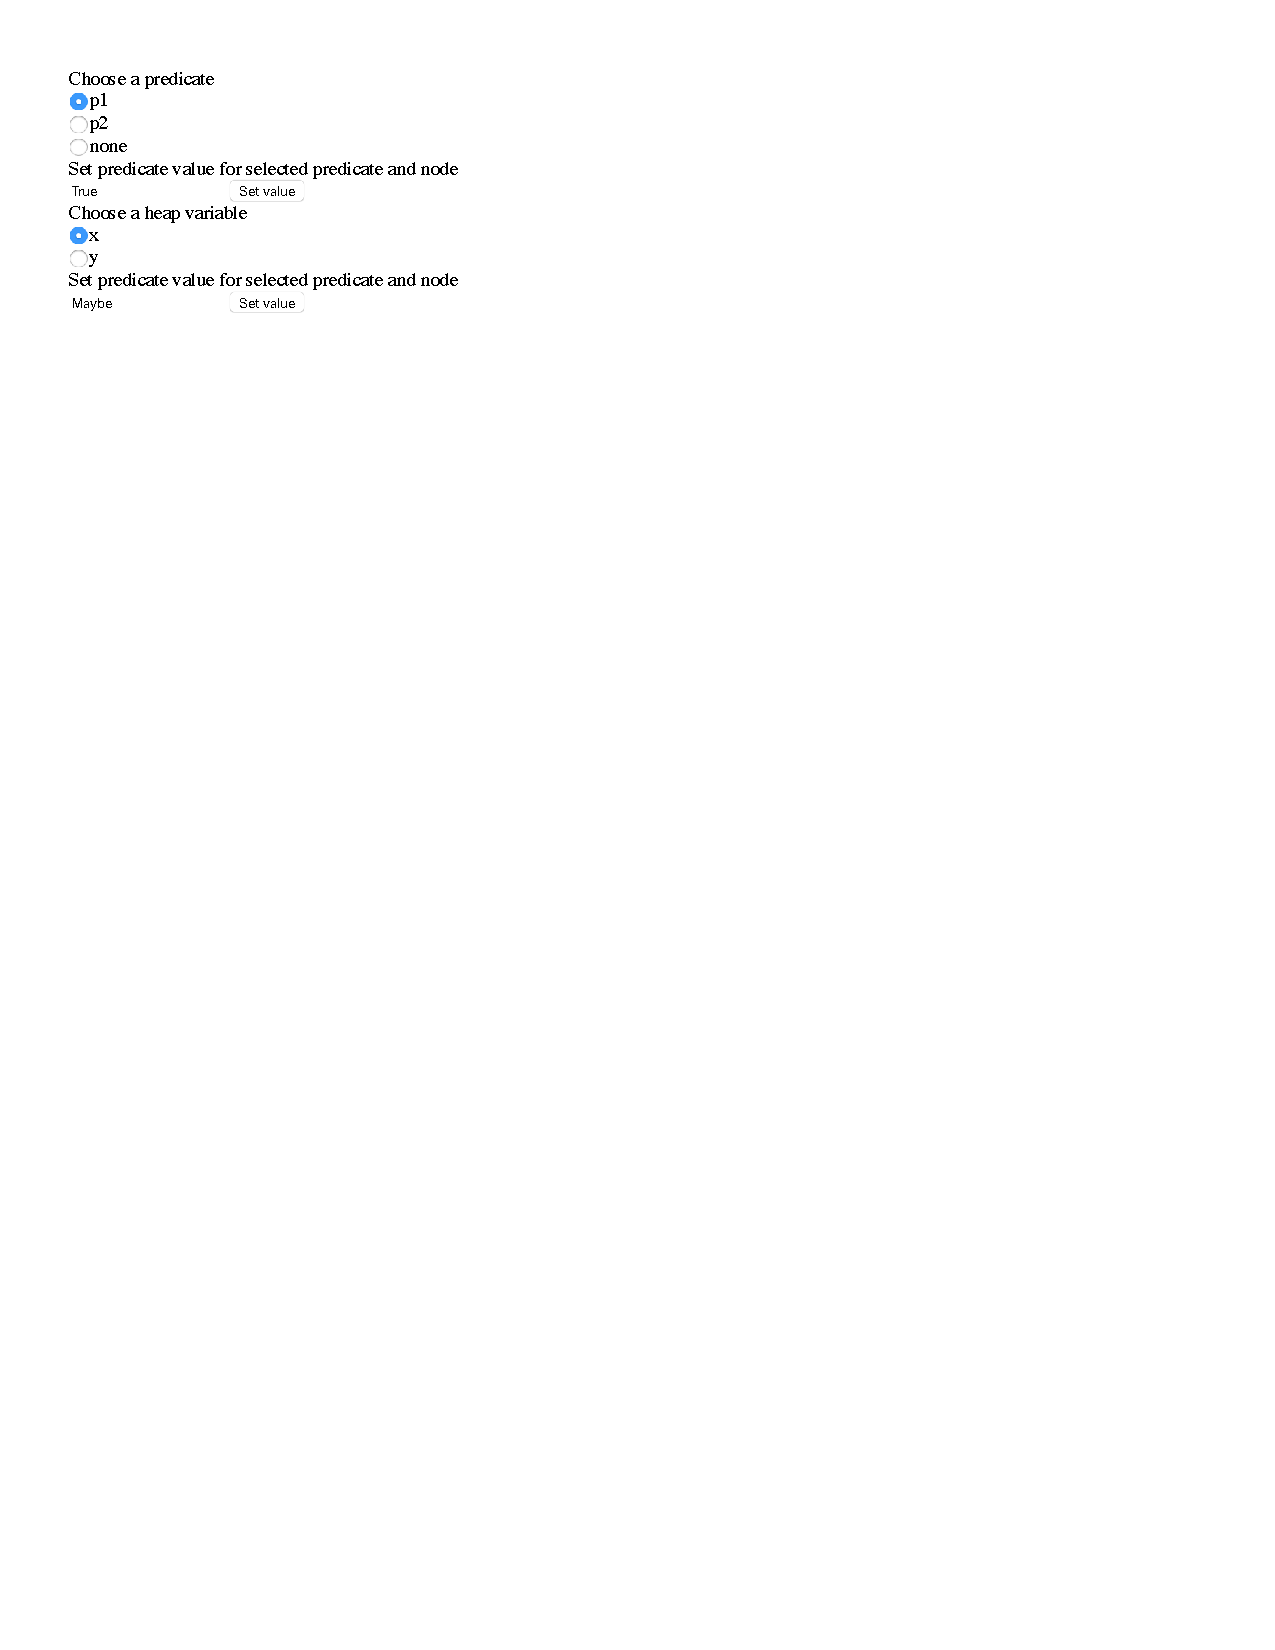
\includegraphics[width=7cm]{fig/predicate-heapvar-val.pdf}
  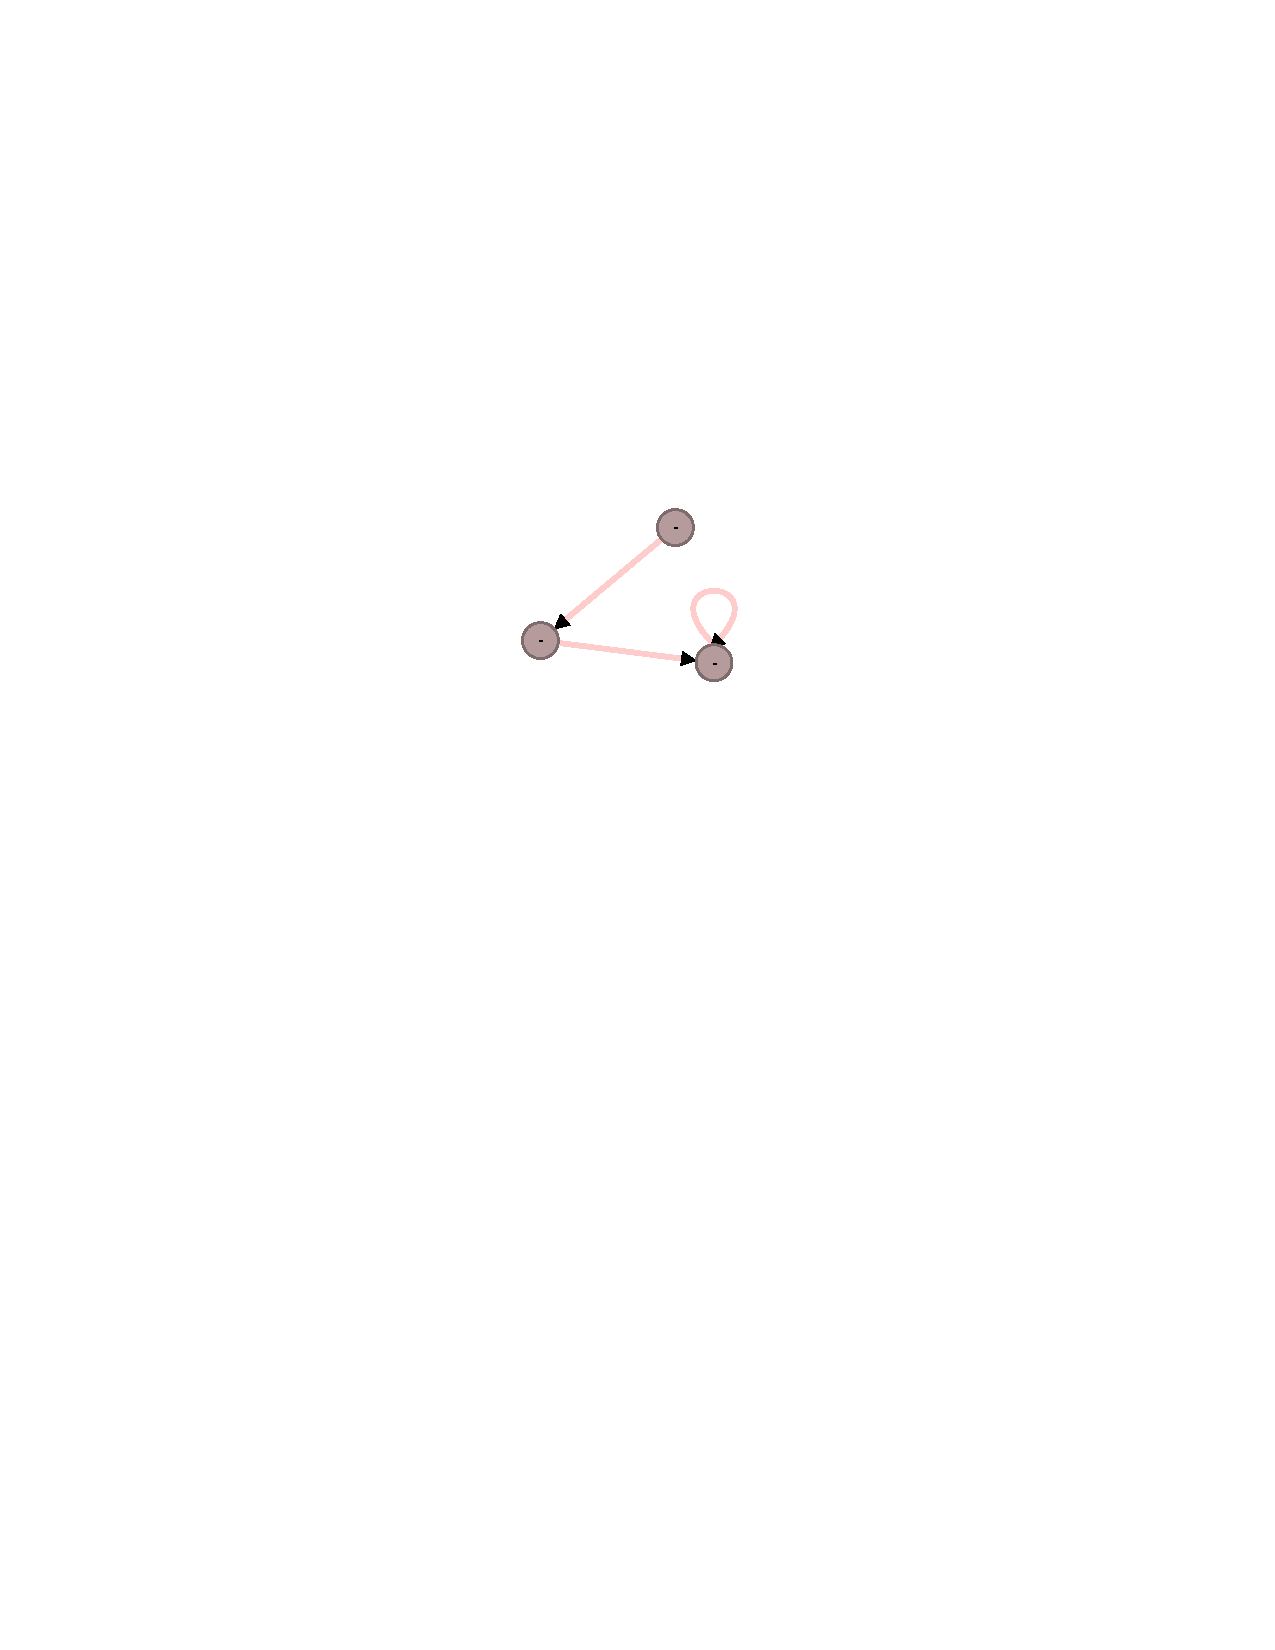
\includegraphics[width=7cm]{fig/basic-graph.pdf}
  \caption{A simple interface to allow the user to graphically draw the heap pattern, and pick values for the predicate and heap variable labeling. The predicates and heap variables have been chosen and populated from a prior analysis. Nodes are represented by circles, and edges as arrows between nodes.
  }
  \label{fig:basic-graph-interface}
\end{figure}

We now dive deeper into all the features provided by the interface, and the user can easily provide a graph pattern matching the formalism described in \autoref{defn:pattern}. One of the important goals of this design is that the user should not have to understand or deal with the formalism itself, but just figures, so that someone with no knowledge of software verification or heap modeling can perform the function of an Oracle.

A heap pattern is a labeled graph represented by the tuple $(\nodesnm, \varlblnm, \predlblnm, \edgesnm, \sigma)$, respectively containing the set of nodes, heap variable labeling, predicate labeling, edges, and summary function. Our interface allows the user to modify the values of each of these attributes of the pattern. We now describe each of these in greater detail.

\subsubsection{Modifying Nodes}
Interacting with nodes is very intuitive:
\begin{itemize}
  \item Click anywhere on empty space to create a new node.
  \item Click on an existing node to select (or unselect) it. Selected nodes appear a lighter shade than unselected nodes. Only up to one node can be selected at a time.
  \item Press the backspace key after selecting a node to delete it. This deletes all edges and resets other attributes relevant to the node.
\end{itemize}

\autoref{fig:modifying-nodes} illustrates the above points clearly.

% Figure illustrating node modification.
\begin{figure}
  \centering
  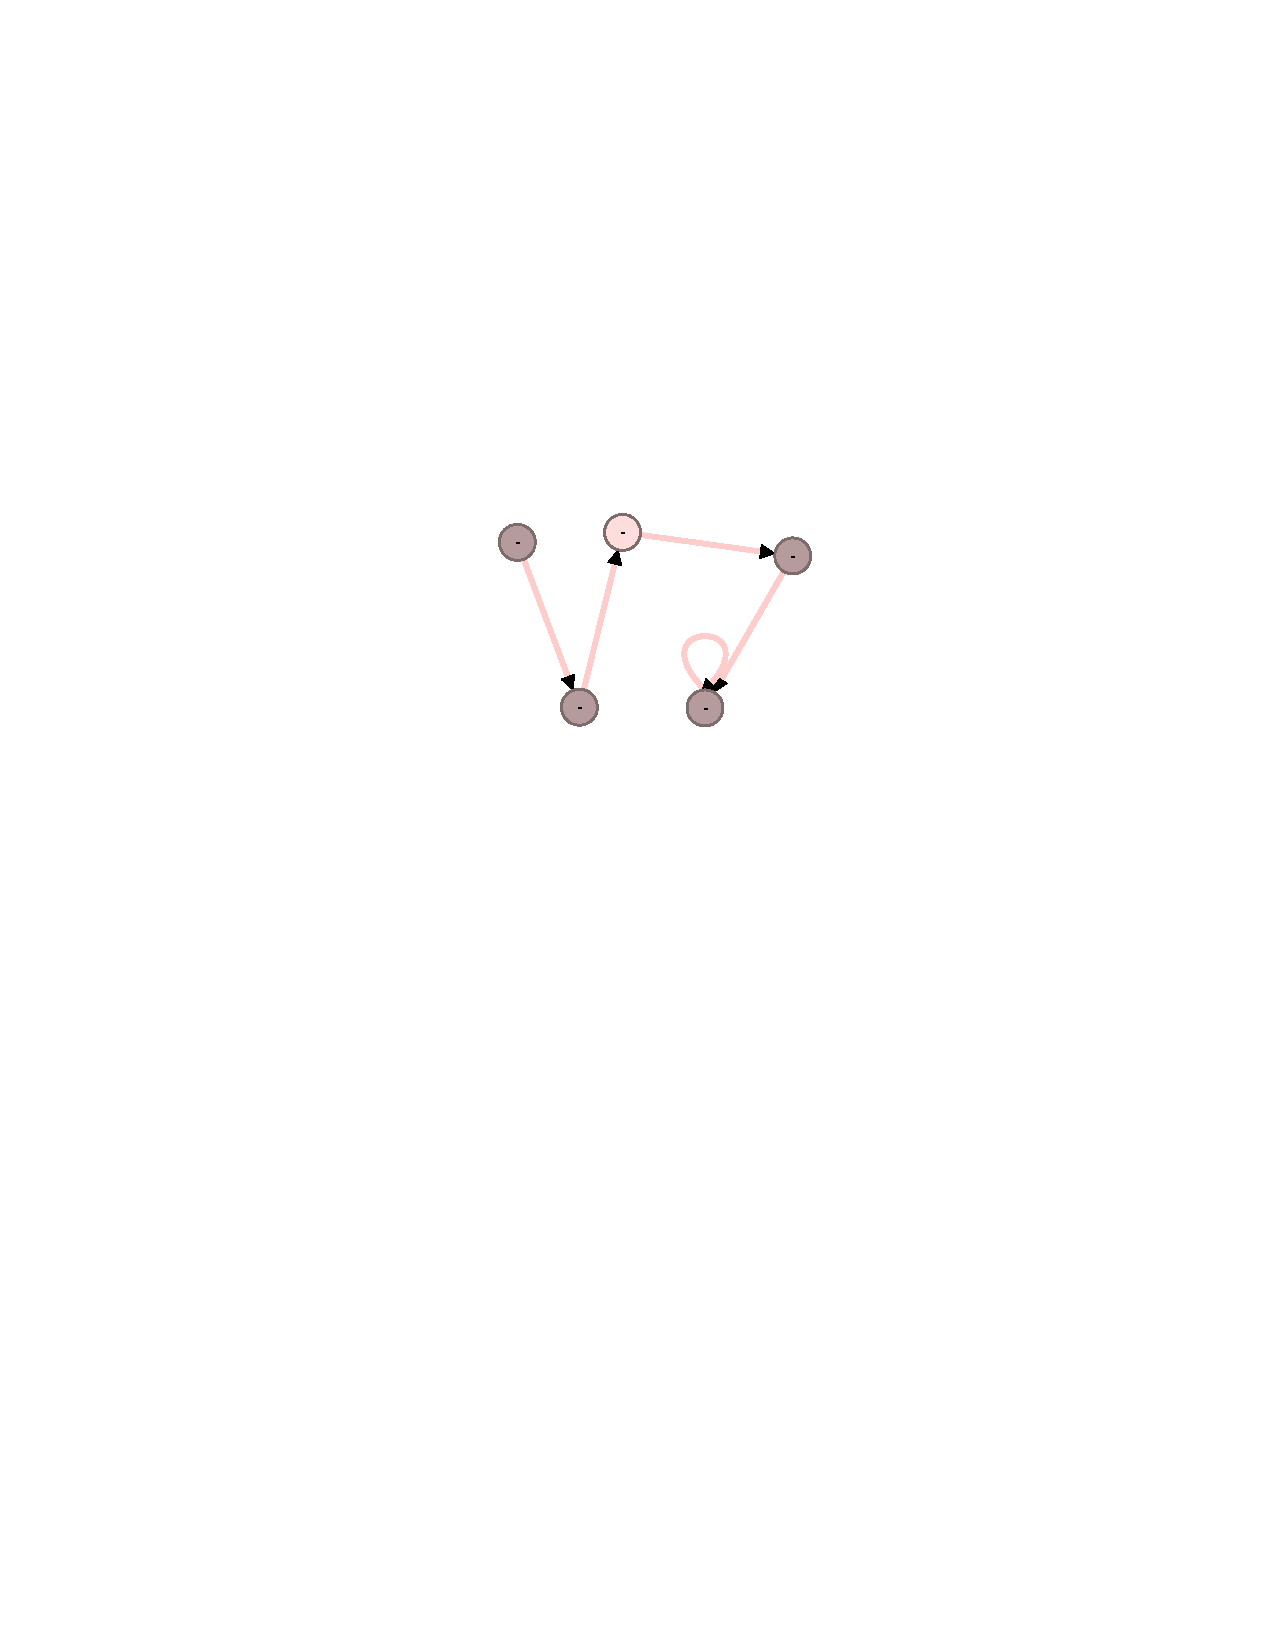
\includegraphics[width=7cm]{fig/nodes-original.pdf}
  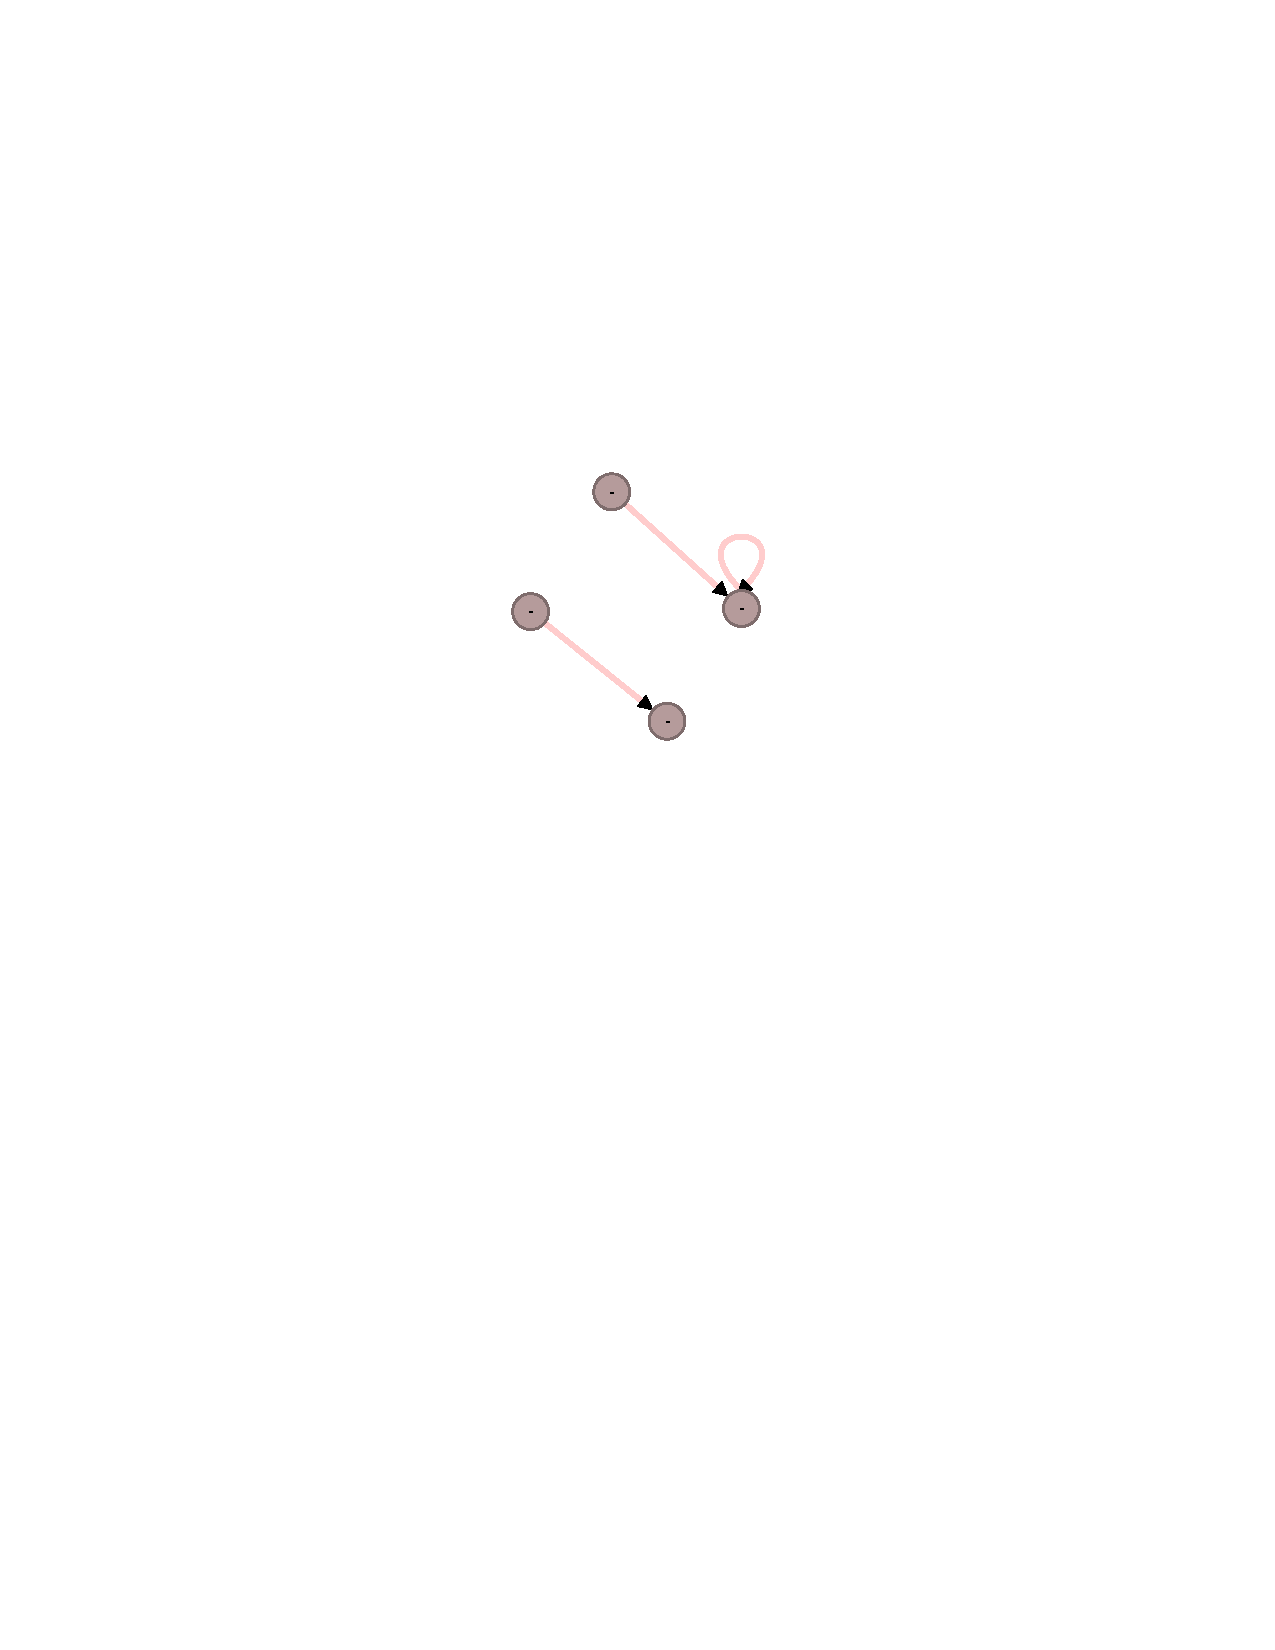
\includegraphics[width=7cm]{fig/nodes-changed.pdf}
  \caption{On the left, the original pattern graph has five nodes, with the middle node selected (indicated by the different color). Pressing the backspace key deletes the node, resulting in the graph on the right.
  }
  \label{fig:modifying-nodes}
\end{figure}

\subsubsection{Modifying the Heap Variable Labeling}
We briefly described the mechanism for updating the heap variable labeling in \autoref{ex:basic-graph-interface}. The interface itself is simple, as shown in \autoref{fig:basic-graph-interface}. In addition, there are some features that make it simpler to keep track of assignments, while preventing user mistakes.

The heap variable labeling is a map $\varlblnm: \nodesnm \times \heapvars \to \threevals$, meaning that each pair of node and heap variable must have a value. To indicate the current assignment, we label the node accordingly. For instance, if the current heap variables are $x, y, z$, and for node $n$, the values of $\varlblnm$ are $\varlblnm(n, x) = \maybe, \varlblnm(n, y) = \true, \varlblnm(n, z) = \false$, then the node will get labeled as $x?y$. The $?$ indicates a $\maybe$ value, the absence of a $?$ indicates $\true$, and absence of the variable altogether indicates $\false$. This keeps the labeling simple, preventing clutter from a large number of $\false$ values, while still making it simple to get a quick idea of the current assignments. Finally, a node with no variable assignments will simply have the label $-$.

We note that $\varlblnm$ is not allowed to have arbitrary assignments. For instance, a variable $x$ cannot be $\true$ for more than one node at the same time. Our interface takes care of such constraints as follows:

\begin{itemize}
  \item Setting a variable to $\true$ for a node sets it to $\false$ for all other nodes automatically.
  \item Setting a variable to $\maybe$ for a node sets it to $\maybe$ for the node where it might currently be $\true$.
\end{itemize}

\autoref{fig:modifying-heap-vars} further illustrates how heap variable labeling works.

% Figure illustrating heap var labeling modification.
\begin{figure}
  \centering
  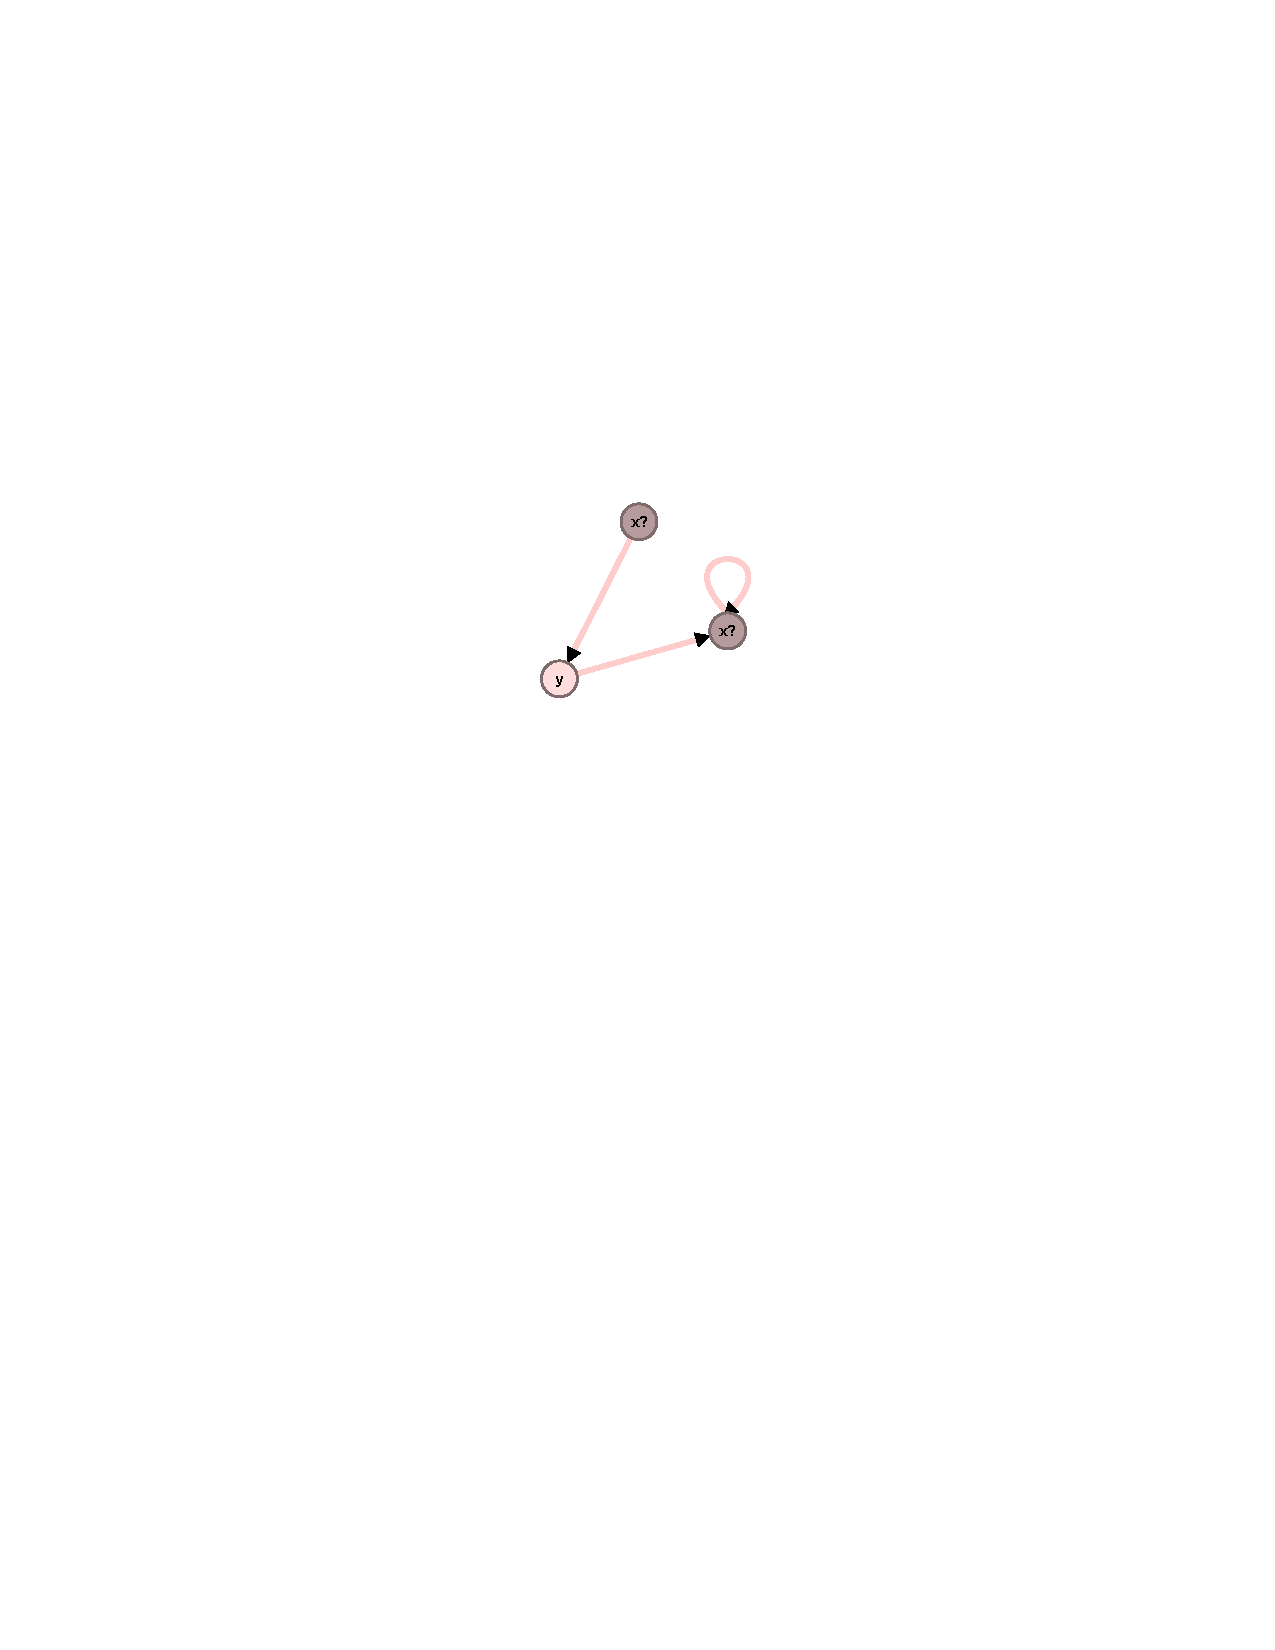
\includegraphics[width=5cm]{fig/heap-var-labeling.pdf}
  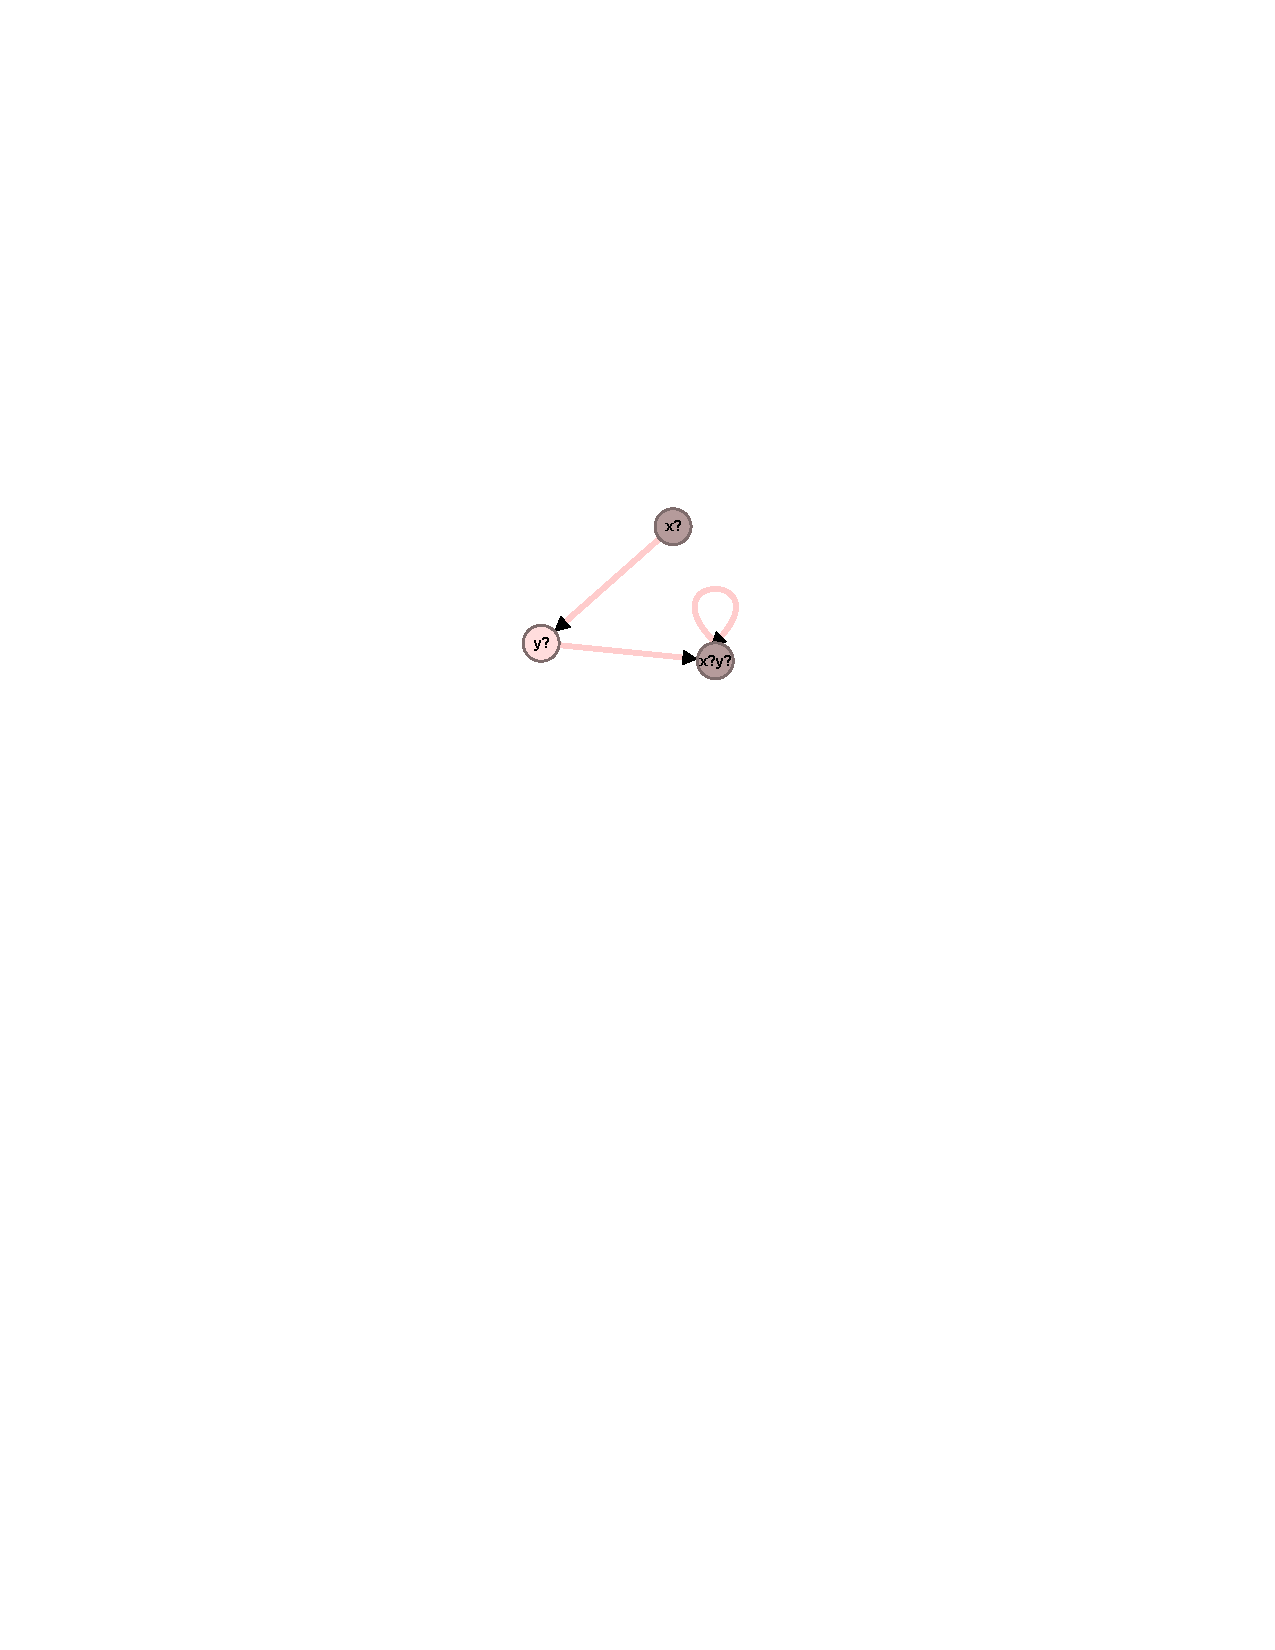
\includegraphics[width=5cm]{fig/heap-var-labeling-2.pdf}
  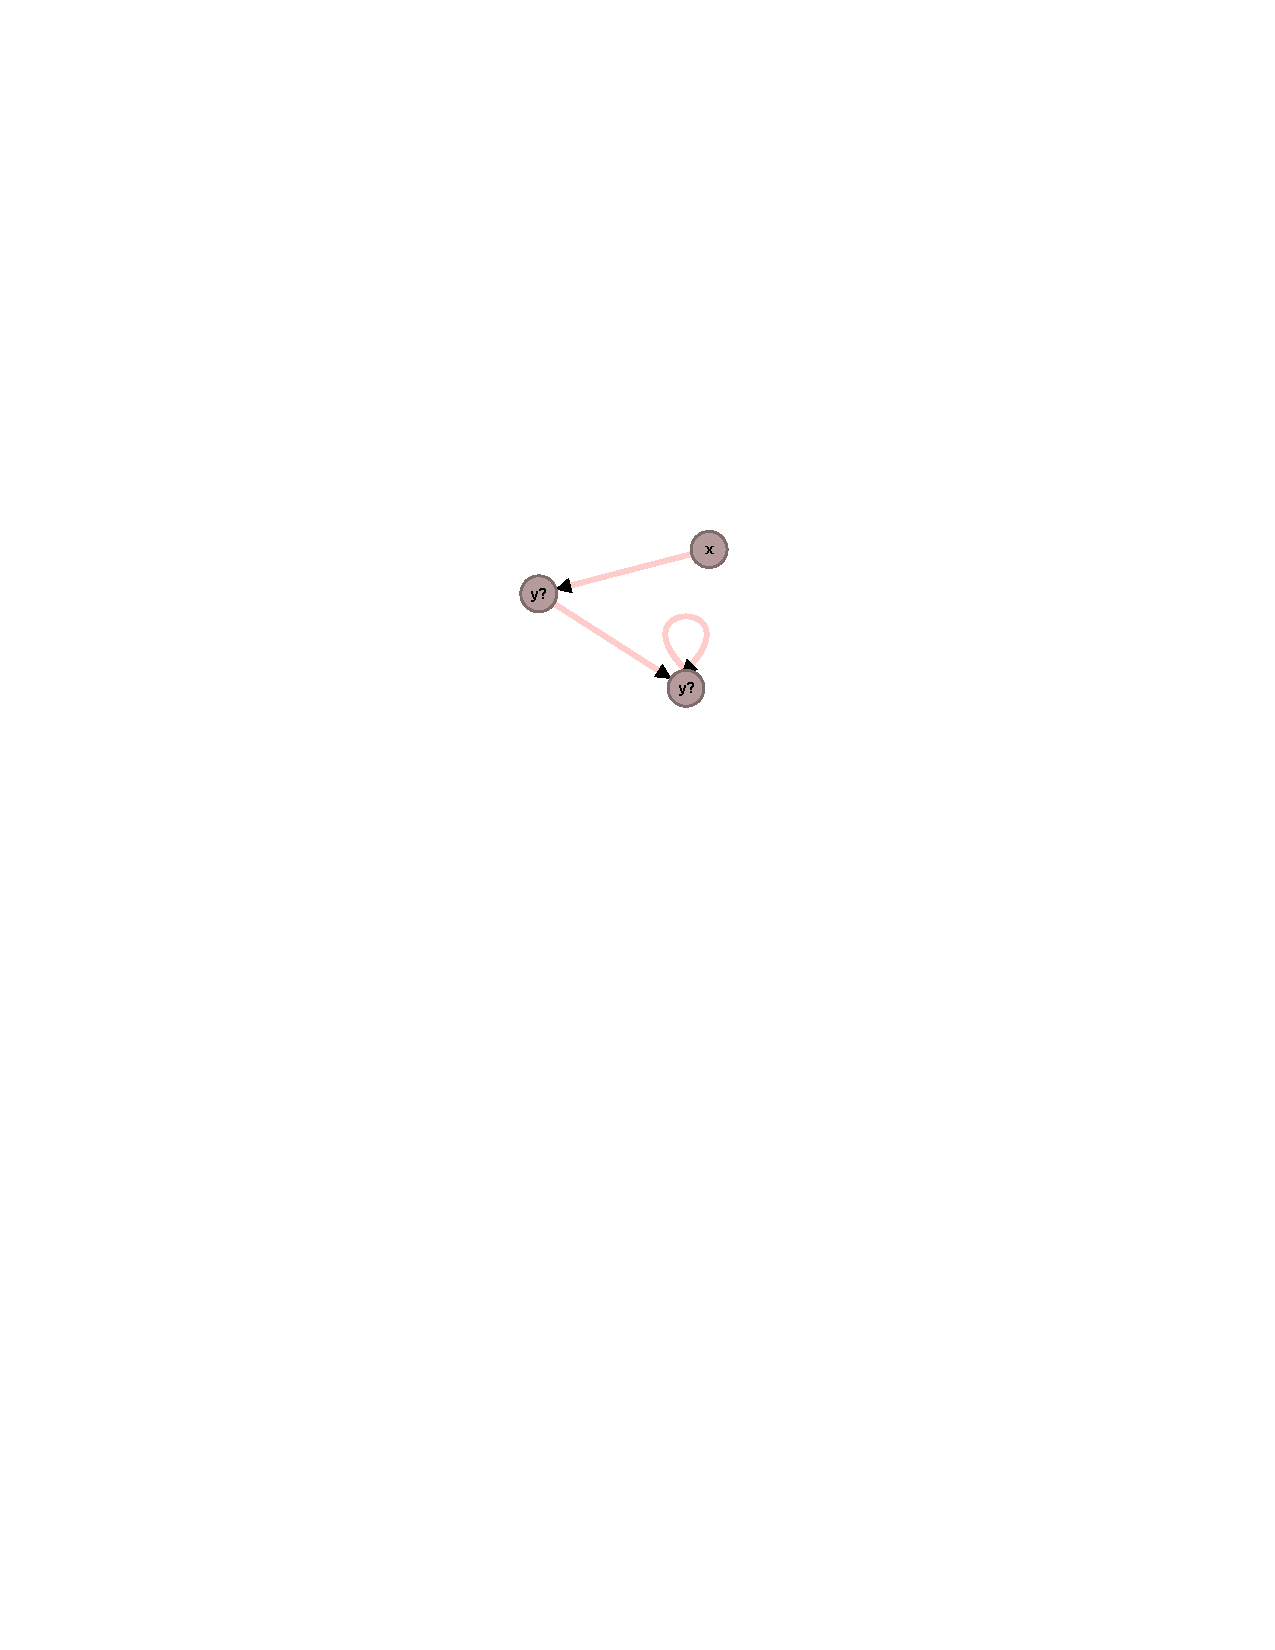
\includegraphics[width=5cm]{fig/heap-var-labeling-3.pdf}
  \caption{The first pattern on the left shows an existing heap variable labeling. We then set the value for $y$ and the node with the self-loop to $\maybe$, which automatically sets the value for $y$ and the selected node to $\maybe$, even though it was $\true$ earlier. Furthermore, in the second pattern, when $x$ is set to $\true$ for the starting node, the value of $x$ is unset for the node with the self-loop.
  }
  \label{fig:modifying-heap-vars}
\end{figure}

\subsubsection{Modifying the Predicate Variable Labeling}
We briefly described the mechanism for updating the predicate variable labeling in \autoref{ex:basic-graph-interface}. The interface itself is simple, as shown in \autoref{fig:basic-graph-interface}. In addition, there are some features that make it simpler to keep track of assignments.

The predicate variable labeling is a map $\predlblnm: \nodesnm \times \predvars \to \threevals$, meaning that each pair of node and predicate variable must have a value. To indicate the current assignment, we use color coding for the nodes - $\predlblnm(n, p) = \true$ imples green, $\predlblnm(n, p) = \false$ imples red, and $\predlblnm(n, p) = \maybe$ implies light pink. Notice that the pattern graph can have multiple predicates available at a time, so the color coding depends on a predicate that is ``live'' at a given time. Predicates can be made live by simply selecting them in the interface shown in \autoref{fig:basic-graph-interface}.

% Figure illustrating pred var modification.
\begin{figure}
  \centering
  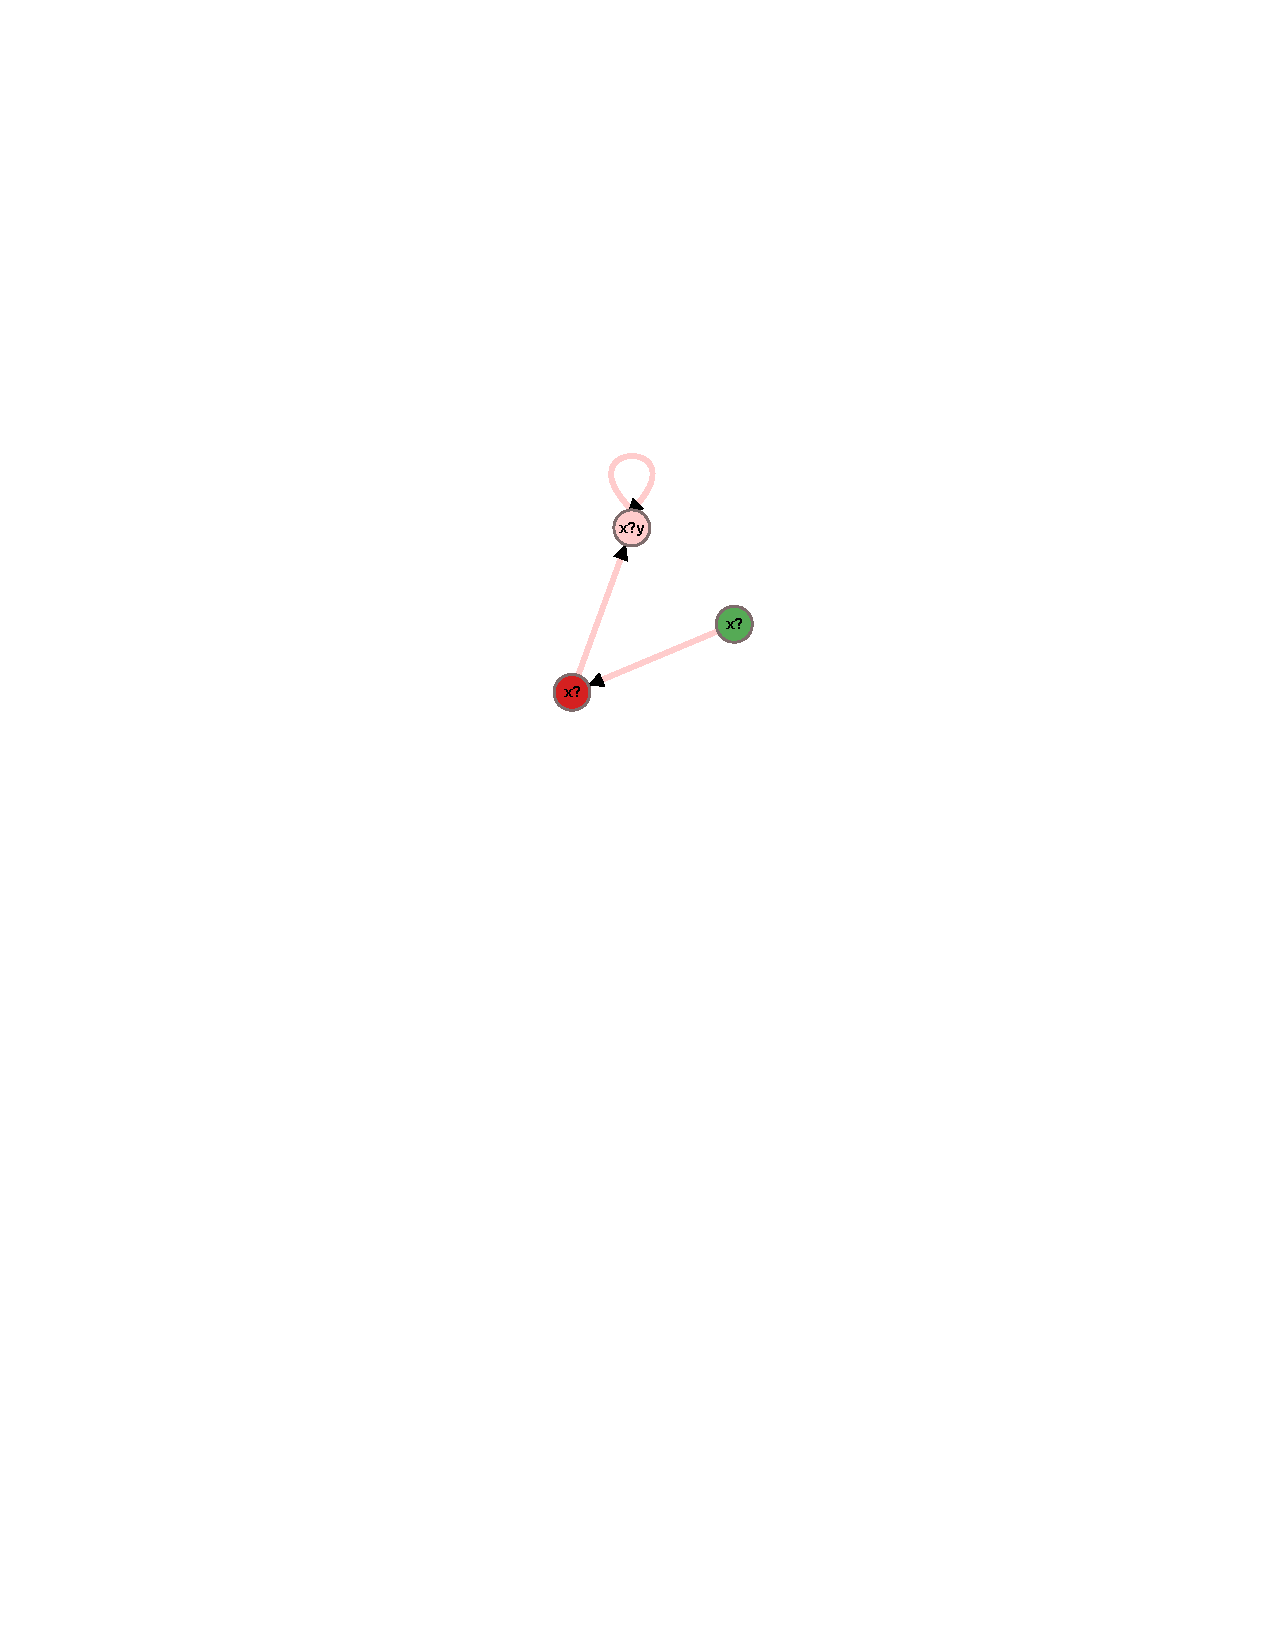
\includegraphics[width=7cm]{fig/predvar.pdf}
  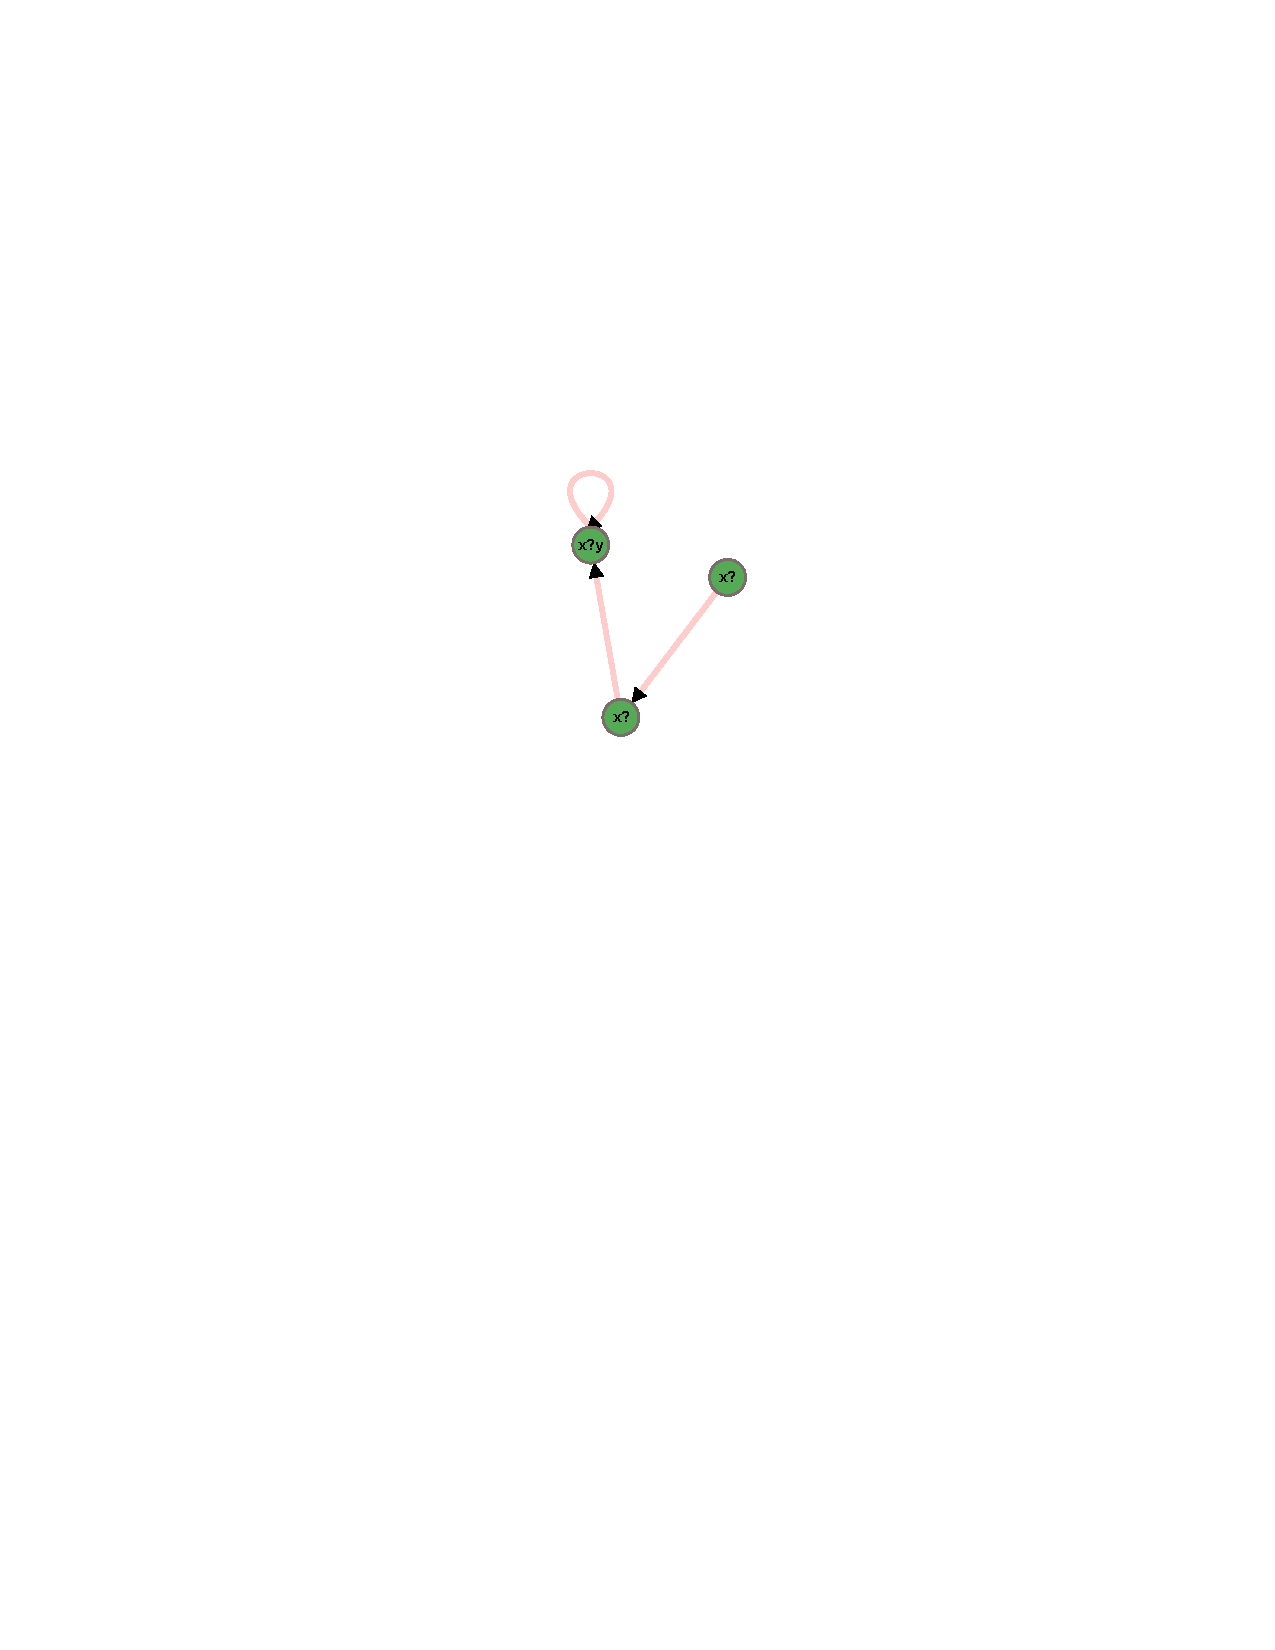
\includegraphics[width=7cm]{fig/predvar2.pdf}
  \caption{On the left, predicate $p1$ is selected, and it has values $\true$, $\false$, and $\maybe$ in order of the arrows, indicated by the appropriate colors. Then we switch the ``live'' predicate to $p2$, which happens to be $\true$ for all nodes, so the color switches to green for each node.}
  \label{fig:modifying-pred-vars}
\end{figure}

\autoref{fig:modifying-pred-vars} illustrates how predicate variable labeling looks.

\subsubsection{Modifying Edges}
Edges are represented by the map $\edgesnm: \nodesnm \times \fields \times \nodesnm \to \threevals$. For our case, since we're only dealing with a single field in the interface, the map can be simplified to $\edgesnm: \nodesnm \times \nodesnm \to \threevals$, meaning that each pair of nodes have an edge between them in either direction. For two nodes $m, n$, $\edgesnm(m, n) = \true$ implies that a green edge exists pointing from $m$ to $n$. $\edgesnm(m, n) = \maybe$ implies that the edge is light pink instead. If $\edgesnm(m, n) = \false$, then this is indicated by the absence of an edge. Once again, this is to make sure that the pattern graph isn't overly cluttered because of too many $\false$ edges. An edge is also a link for the force-directed graph in D3.

Interacting with edges is fairly simple:
\begin{itemize}
  \item Drag the mouse from a node to another to create an edge between them, in the direction of dragging.
  \item Click on an existing edge to select (or unselect) it. Selected edges appear dotted, as opposed to solid for unselected edges. Only up to one edge can be selected at a time.
  \item Press the backspace key after selecting a edge to delete it.
  \item Pressing the M key for a selected edge toggles between $\true$ and $\maybe$ values for that edge (respectively green and light pink).
  \item Pressing the R key for a selected node creates a self-loop on that node. Each node can have only one self-loop, and all edge interactions work for it just like other edges.
\end{itemize}

Edges are normally straight, but bidirectional edges are rounded for better visibility. \autoref{fig:modifying-edges} illustrates how the interface allows for interaction with edges.

Just like $\varlblnm$, $\edgesnm$ is not allowed to have arbitrary assignments. For instance, a $\true$ edge going out from a node implies that there cannot be any other edge going out of the same node. Our interface takes care of such constraints as follows:

\begin{itemize}
  \item Setting an edge (from node $m$ to $n$) to $\true$ sets all outgoing edges from $m$ $\false$ automatically i.e. deletes them.
  \item Setting an edge (from node $m$ to $n$) to $\maybe$ sets any $\true$ outgoing edge from $m$ to $\maybe$ automatically.
\end{itemize}

\autoref{fig:edge-constraints} illustrates how constraints on $\edgesnm$ are enforced by the interface.

\subsubsection{Modifying the Summary Function}
The summary function $\sigma: \nodesnm \to \bools$ indicates where a node is a summary node. Our interface indicates summary nodes by making them larger than other nodes. Selecting a node and pressing the S key toggles the value of $\sigma$ for that node. \autoref{fig:summary-nodes} illustrates an example of this.

\subsection{User Interaction}
We describe the user's workflow while interacting with the interface.